\begin{figure}
  \centering
  \definecolor{cs-PipelineColor}{rgb}{1.0,0.901,0.805}
  \definecolor{cs-ClusteredColor}{rgb}{0.7,0.9,1.0}

  
  
  % Styles
  % --------------------------------------------------------------------------
  \tikzstyle{cs-algorithm-base}=[rectangle,
                                 draw=black,
                                 rounded corners,
                                 text centered,
                                 minimum height=1.5cm,
                                ]
  \tikzstyle{cs-pipeline}=[cs-algorithm-base,
                        fill={cs-PipelineColor},
                        minimum width=7cm]
\tikzstyle{clustered}=[cs-algorithm-base,
                     fill={cs-ClusteredColor},
                     minimum width=15cm]
  \tikzstyle{cs-anchor}=[minimum width=7cm, minimum height=1.5cm]
  \begin{adjustbox}{minipage=\textwidth, scale=0.6}
 
  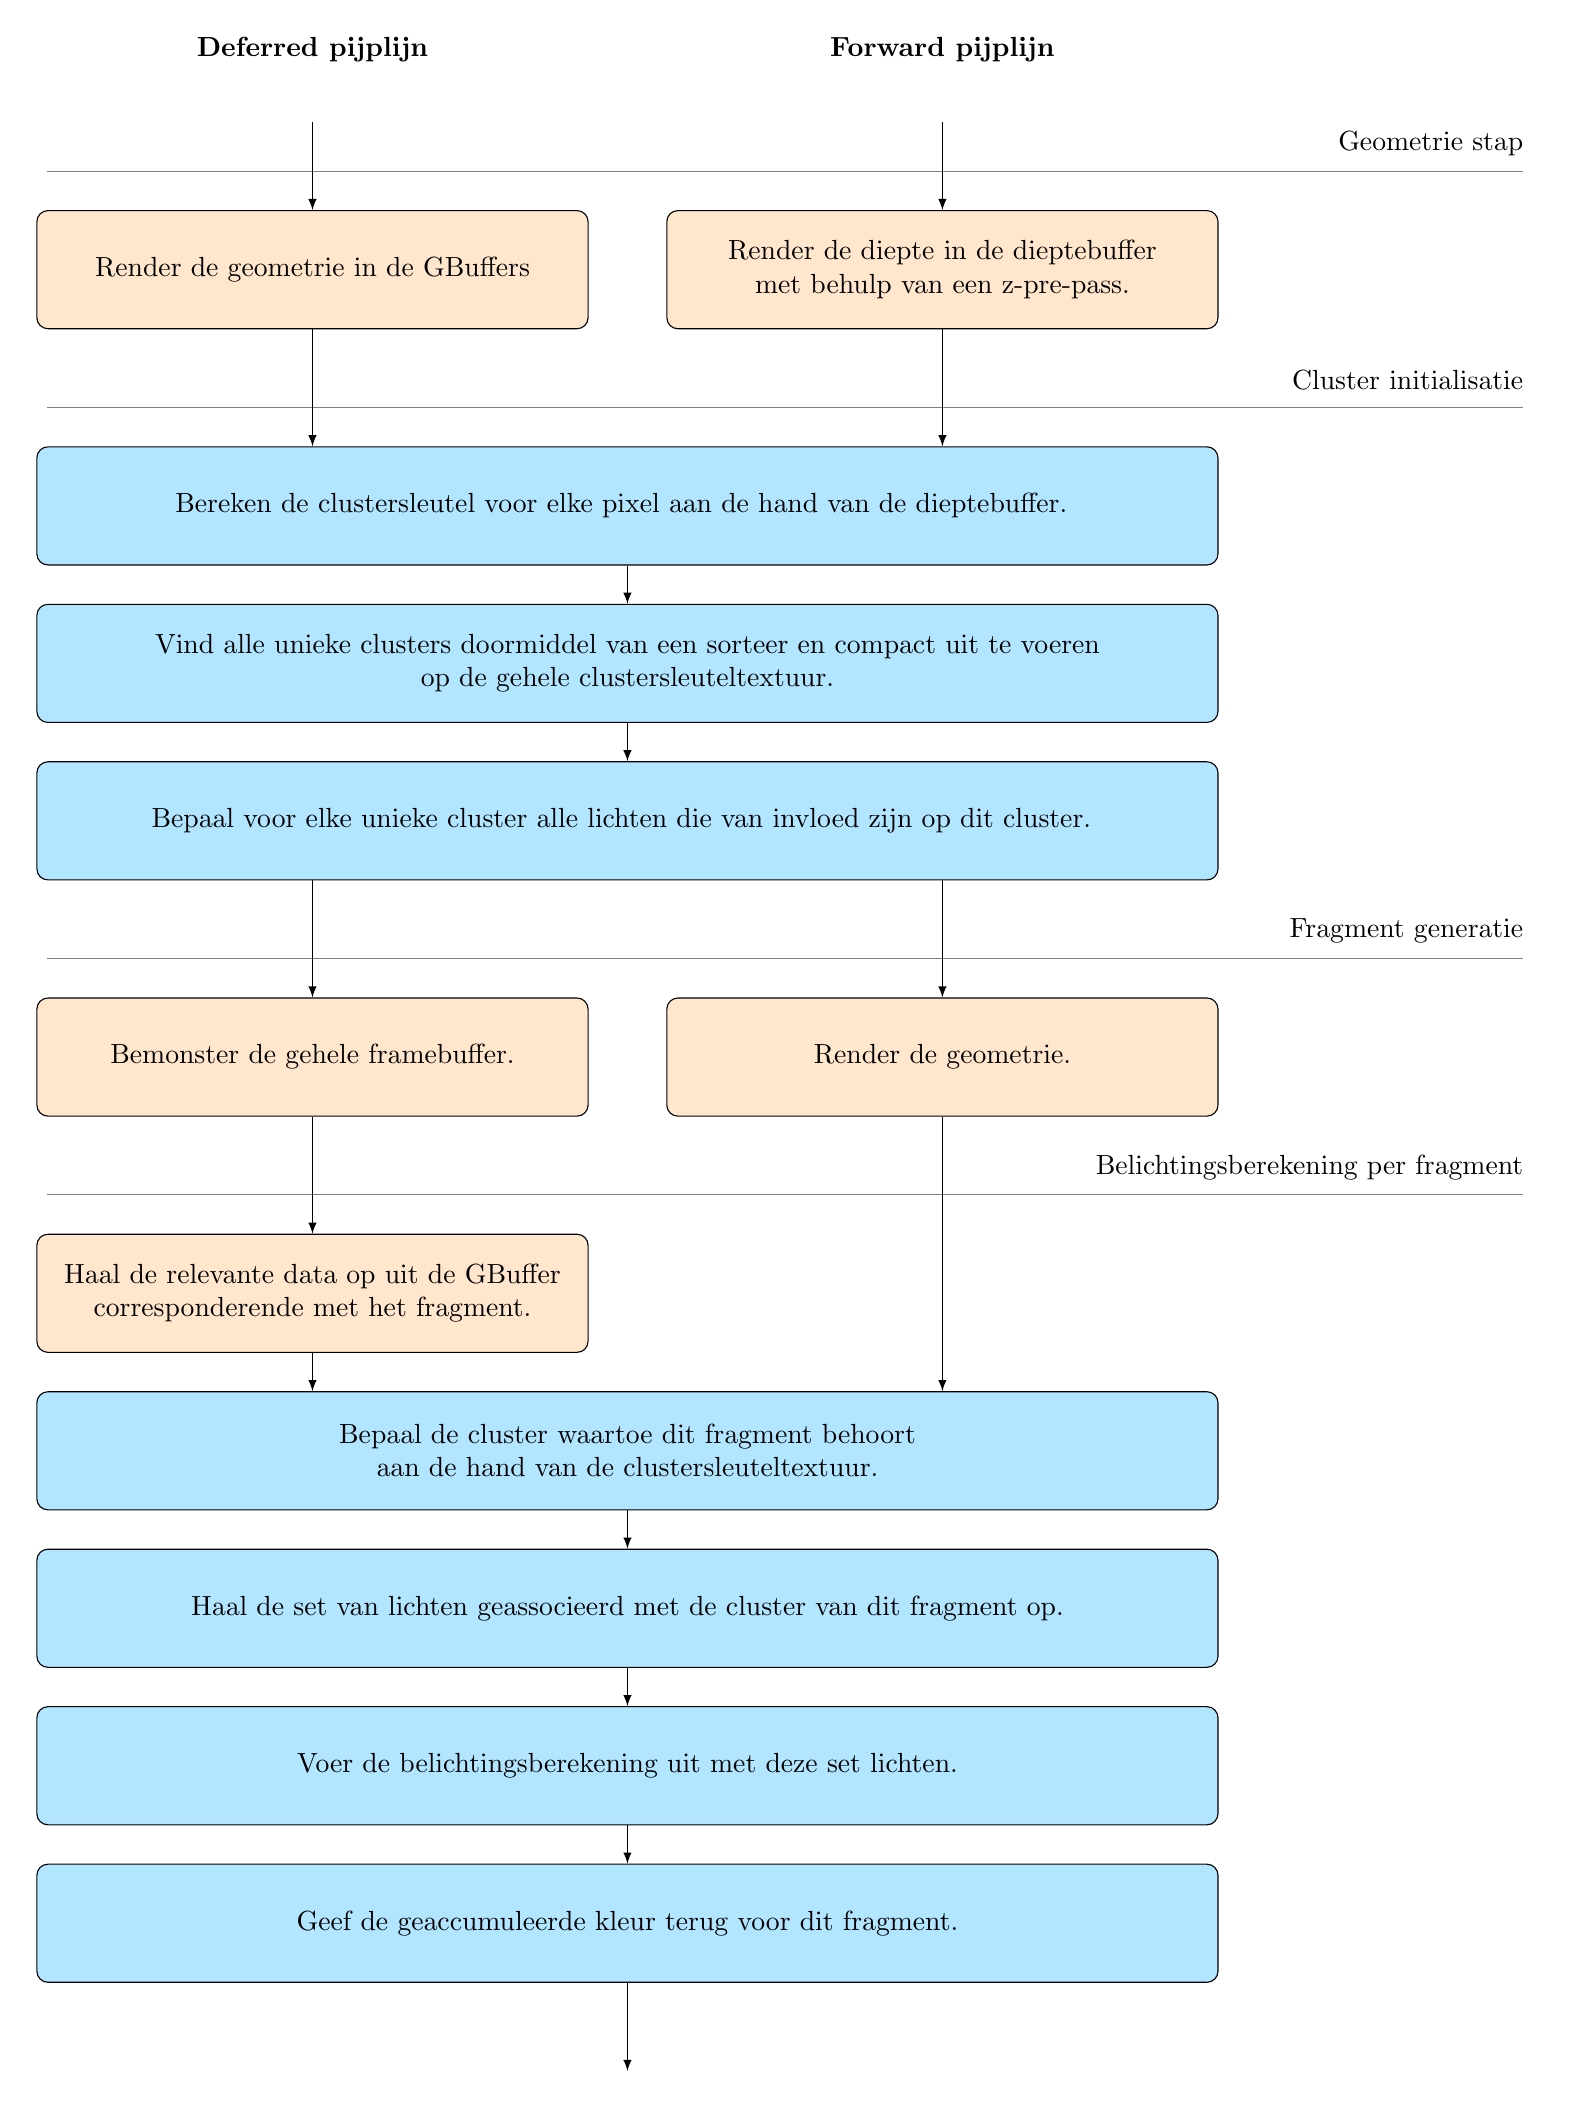
\begin{tikzpicture}[node distance=1.5cm
                      every node/.style={fill=white}, align=center]
    % Steps
    % --------------------------------------------------------------------------
    \node at (-4,  3.8) (deferred_text) [] {\textbf{Deferred pijplijn}};
    \node at ( 4,  3.8) (forward_tex)   [] {\textbf{Forward pijplijn}};
   
    \node at (-4,  3.0) (deferred_in)   [] {};
    \node at ( 4,  3.0) (forward_in)    [] {};
   
    % ------------------------------------------------------------------------
    \node at (-4,  1.0) (deferred_step0) [cs-pipeline] {Render de geometrie in de GBuffers};
    \node at (4,  1.0) (forward_step0) [cs-pipeline] {Render de diepte in de dieptebuffer\\met behulp van een z-pre-pass.};
   
    % ------------------------------------------------------------------------
    \node at (-4,  -2) (anchor_deferred_step1) [cs-anchor] {};
    \node at ( 4,  -2) (anchor_forward_step1)  [cs-anchor] {};
 
    \node at (0.0, -2) (step1) [clustered] { Bereken de clustersleutel voor elke pixel aan de hand van de dieptebuffer. };
    \node at (0.0, -4) (step2) [clustered] { Vind alle unieke clusters doormiddel van een sorteer en compact uit te voeren\\
                                                                 op de gehele clustersleuteltextuur. };
    \node at (0.0, -6) (step3) [clustered] { Bepaal voor elke unieke cluster alle lichten die van invloed zijn op dit cluster. };
   
    % ------------------------------------------------------------------------
     \node at (-4, -6) (anchor_deferred_step3) [cs-anchor] {};
     \node at ( 4, -6) (anchor_forward_step3)  [cs-anchor] {};
 
     \node at (-4,  -9) (deferred_step4) [cs-pipeline] {Bemonster de gehele framebuffer.};
     \node at ( 4,  -9) (forward_step4)  [cs-pipeline] {Render de geometrie.};
   
    % ------------------------------------------------------------------------
     \node at (-4, -12) (deferred_step5) [cs-pipeline] {Haal de relevante data op uit de GBuffer\\
                                                                               corresponderende met het fragment.};
 
    \node at (-4, -14) (anchor_deferred_step6) [cs-anchor] {};
    \node at ( 4, -14) (anchor_forward_step6)  [cs-anchor] {};
   
      \node at ( 0, -14) (step6) [clustered] { Bepaal de cluster waartoe dit fragment behoort\\ aan de hand van de clustersleuteltextuur.};
      \node at ( 0, -16) (step7) [clustered] { Haal de set van lichten geassocieerd met de cluster van dit fragment op.};
    \node at ( 0, -18) (step8) [clustered] { Voer de belichtingsberekening uit met deze set lichten.};
    \node at ( 0, -20) (step9) [clustered] { Geef de geaccumuleerde kleur terug voor dit fragment.};
    \node at ( 0, -22) (out) [] { };
   
     % Step lines
    % --------------------------------------------------------------------------
    \node at ( -7.5, 2.25) (line_1_l) [] {};
    \node at ( 11.5, 2.25) (line_1_r) [] {};
    \draw[gray] (line_1_l) -- (line_1_r);
    \node at ( 11.5, 2.60) (line_1_text) [anchor=east] {Geometrie stap};
 
    \node at ( -7.5, -0.75) (line_2_l) [] {};
    \node at ( 11.5, -0.75) (line_2_r) [] {};
    \draw[gray] (line_2_l) -- (line_2_r);
    \node at ( 11.5, -0.40) (line_2_text) [anchor=east] {Cluster initialisatie};
 
    \node at ( -7.5, -7.75) (line_3_l) [] {};
    \node at ( 11.5, -7.75) (line_3_r) [] {};
    \draw[gray] (line_3_l) -- (line_3_r);
    \node at ( 11.5, -7.40) (line_3_text) [anchor=east] {Fragment generatie};
 
    \node at ( -7.5, -10.75) (line_4_l) [] {};
    \node at ( 11.5, -10.75) (line_4_r) [] {};
    \draw[gray] (line_4_l) -- (line_4_r);
    \node at ( 11.5, -10.40) (line_4_text) [anchor=east] {Belichtingsberekening per fragment};
   
   
    % Arrows
    % --------------------------------------------------------------------------
    \draw[-latex] (deferred_in)    -- (deferred_step0);
    \draw[-latex] (forward_in)     -- (forward_step0);
    \draw[-latex] (deferred_step0) -- (anchor_deferred_step1);
    \draw[-latex] (forward_step0)     -- (anchor_forward_step1);
 
    \draw[-latex] (step1) -- (step2);
    \draw[-latex] (step2) -- (step3);
 
    \draw[-latex] (anchor_deferred_step3) -- (deferred_step4);
    \draw[-latex] (anchor_forward_step3)  -- (forward_step4);
 
    \draw[-latex] (deferred_step4) -- (deferred_step5);
    \draw[-latex] (deferred_step5) -- (anchor_deferred_step6);
   
    \draw[-latex] (forward_step4) -- (anchor_forward_step6);
 
    \draw[-latex] (step6) -- (step7);
    \draw[-latex] (step7) -- (step8);
    \draw[-latex] (step8) -- (step9);
    \draw[-latex] (step9) -- (out);
   
  \end{tikzpicture}
  \end{adjustbox}
  \caption{Het Tiled Shading algoritme voor de Forward en Deferred pijplijn.}
  \label{fig:ts-algorithm}
\end{figure}
